%
% LAYOUT.TEX - Kurzbeschreibung von PA 88-10-04 (LaTeX)
%                                      99-03-20
%
%  Updated for REFMAN.CLS (LaTeX2e)
%
\documentclass[twoside,a4paper]{refart}
%\documentclass[pagesize,twoside,a5paper,smallborder,10pt]{refart}
\usepackage[T1]{fontenc}
\usepackage{ae} % CM-Zeichens"atze mit T1 encoding
\usepackage{makeidx}
\usepackage{ifthen}
\usepackage{german}
%\usepackage{showidx}
\usepackage[pdftex]{graphicx}
\usepackage{wrapfig}
\usepackage{hyperref}

\DeclareRobustCommand\cs[1]{\texttt{\char`\\#1}}
\def\bs{\char'134 } % backslash in \tt font.
\newcommand{\zB}{z.\,B.}
\newcommand{\dH}{d.\,h.}  

\title{Zahnriemenwechsel VW 2.0 TDI CAAB}
\author{TX-BOARD.de \\Nutzer 3pleL \\}

\date{}
\emergencystretch1em  % F"ur TeX <3.0 auskommentieren!

%\pagestyle{footings}
%\pagestyle{headings}
%\pagestyle{myfootings}
\markboth{Layout-"Anderungen mit \textrm{\LaTeX}}%
         {Layout-"Anderungen mit \textrm{\LaTeX}}

\makeindex % Dies nur als Demonstration, das jetzt auch ein Index
           % m"oglich ist :-)
% Bei Marginlabels mu"s der Index *vor* dem Label stehen.

% Es ist notwendig die Umlaute in der TeX-Schreibweise zu schreiben,
% da der german.sty sie sonst in etwas verwandeln w"urde, mit dem
% MakeIndex nicht zurecht kommt.


\setcounter{tocdepth}{2}
\settextfraction{0.7}

\begin{document}
\maketitle

\begin{abstract}
	Der vorliegende Erfahrungsbericht beschreibt den Wechsel des Zahnriemen an einem VW T5 Facelift mit 2.0l TDI Dieselmotor (CAAB). Er basiert überwiegend auf verstreuten Posts hier im Forum, der original Reparaturanleitung und einigen Youtube Videos. Er ersetzt \textbf{NICHT} die originale Anleitung, die über \href{https://erwin.volkswagen.de/erwin/showHome.do}{Erwin} verfügbar ist. Auch ersetzt dieser Bericht nicht den gesunden Menschenverstand und sorgfältigstes Arbeiten. 
	Da ich kein ausgebildeter Mechaniker bin, betrachte man diesen Bericht nicht als der Weisheit letzten Schluss sondern lediglich als ergänzende Notizen!
	
	Mein besonderer Dank gilt den Forennutzern Nendoro, Slaughtercult, KS-RMB, Schumo, T5erFAN für ihre Unterstützung. 
\end{abstract}

\tableofcontents

\newpage


%%%%%%%%%%%%%%%%%%%%%%%%%%%%%%%%%%%%%%%%%%%%%%%%%%%%%%%%%%%%%%%%%%%%

\section{Einleitung}

\subsection{Benötigtes Werkzeug}
\begin{itemize}
	\item Wagenheber + Holzklötze
	\item Unterstellböcke
	\item Rätschenkasten 
	\item Vielzahn Nuss 19mm 
	\item M8, M10 XZN Bits
	\item Absteckwerkzeug 2.0 TDI 
	\item Drehmomentschlüssel
	\item Schlauchschellenzange
	\item Gegenhalter
	\item ggf. rückschlagsfreier Schonhammer
	\item Licht
	\item VCDS
\end{itemize}

\marginlabel{Kommentar:}
Bei meinem Absteckwerkzeug war nur ein Absteckdorn für die Nockenwelle mit dabei. Für die Hochdruckpumpe wird ebenfalls ein Dorn benötigt, ich habe einen 6mm Bohrer verwendet.

Ein Schlagschrauber ist nicht zwingend nötig, vereinfacht aber einiges.

\subsection{Benötigte Ersatzteile}
\begin{itemize}
	\item Zahnriemensatz inkl. Wasserpumpe, Umlenkrollen ect. (Contitech CT1139WP6)
	\item Schrauben Wasserpumpe 3x N90945002
	\item Schrauben Hochdruckpumpe 3x N91180301
	\item Schrauben Motorträger N10666601, N10655802, N10680203, N10661101, 3x N91023602
	\item Schrauben Riemenscheibe Schwingungsdämpfer 4x N91048804
	\item Kühlmittel
\end{itemize}

\marginlabel{Kommentar:}
Bei dem Contitech Satz waren die Schrauben für die Nockenwelle, Stehbolzen ect. mit dabei.

\subsection{Video-Quellen}
Youtube Videos: \\
Englische Videos zum T5 \\
\href{https://www.youtube.com/watch?v=lM7_e-wfeLw}{Teil 1} - Benötigte Werkzeuge\\
\href{https://www.youtube.com/watch?v=5waO83BzXO8}{Teil 2} - Verkleidungen abbauen\\
\href{https://www.youtube.com/watch?v=JyRyLn6IAqA}{Teil 3} - Zahnriemenwechsel\\
\href{https://www.youtube.com/watch?v=LfvovYmEzTM}{Teil 4} - Zusammenbau\\

Gutes Video zum Einstellen der Steuerzeiten sowie der Anwendung des Gegenhalters\\
\href{https://www.youtube.com/watch?v=io7AP5-M3bM}{Audi A4 2.0 TDI Zahnriemenwechsel}\\
\clearpage
\section{Vorbereitung}
Ganz nach rechts einlenken, den Wagen aufbocken. Ich habe ihn am Ende des Aggregateträgers (Abb. \ref{fig:aggregateträger}) auf einem Abstellbock abgestellt.
Anschließend das Rad abnehmen. Daraufhin lässt sich der Spritzschutz ausbauen. Damit hat man gute Sicht und ein bisschen mehr Platz. Bei der Gelegenheit kann man gleich den Dreck im Radlauf entfernen.
Wer später eine Sauerei mit Kühlwasser vermeiden möchte kann jetzt den Kühlmittelkreislauf leeren (vgl. So wird's gemacht - Band 134, S. 194).
\begin{figure}[htb]
	\begin{center}
		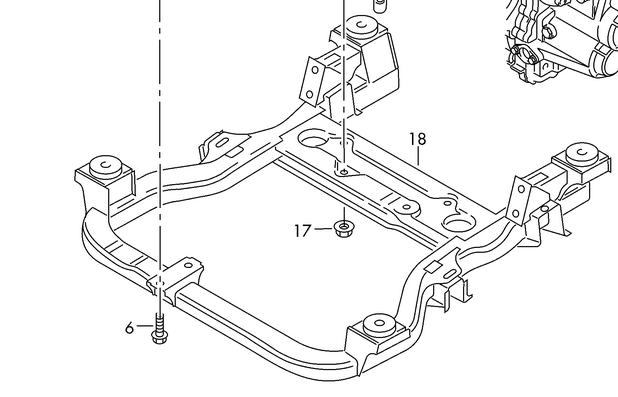
\includegraphics[width=\textwidth]{Aggregatetraeger}
		\caption{Aggregateträger}
		\label{fig:aggregateträger}
	\end{center}
\end{figure}

\subsection{Motor abfangen}
Laut Reparaturleitfaden muss der Motor von oben abgefangen werden. In Ermangelung einer passenden Vorrichtung habe ich den Motor von unten an der Ölwanne mit dem Wagenheber abgestützt. Dabei ist zum Schutz der Ölwanne die Auflagefläche des Hebers durch ein geeigneten Holzbalken zu vergrößern!
 
\newpage
\section{Platz schaffen}
Ansaugrohr mitsamt Luftmassemesser (Abb. \ref{fig:luftfilerkasten} -6-) abbauen, die Stecker können bequem hinter den Klimaleitungen verstaut werden. Anschließend das Rohr nach oben drehen und unter dem Wasserkasten festklemmen.\\

\begin{figure}[htb]
	\begin{center}
		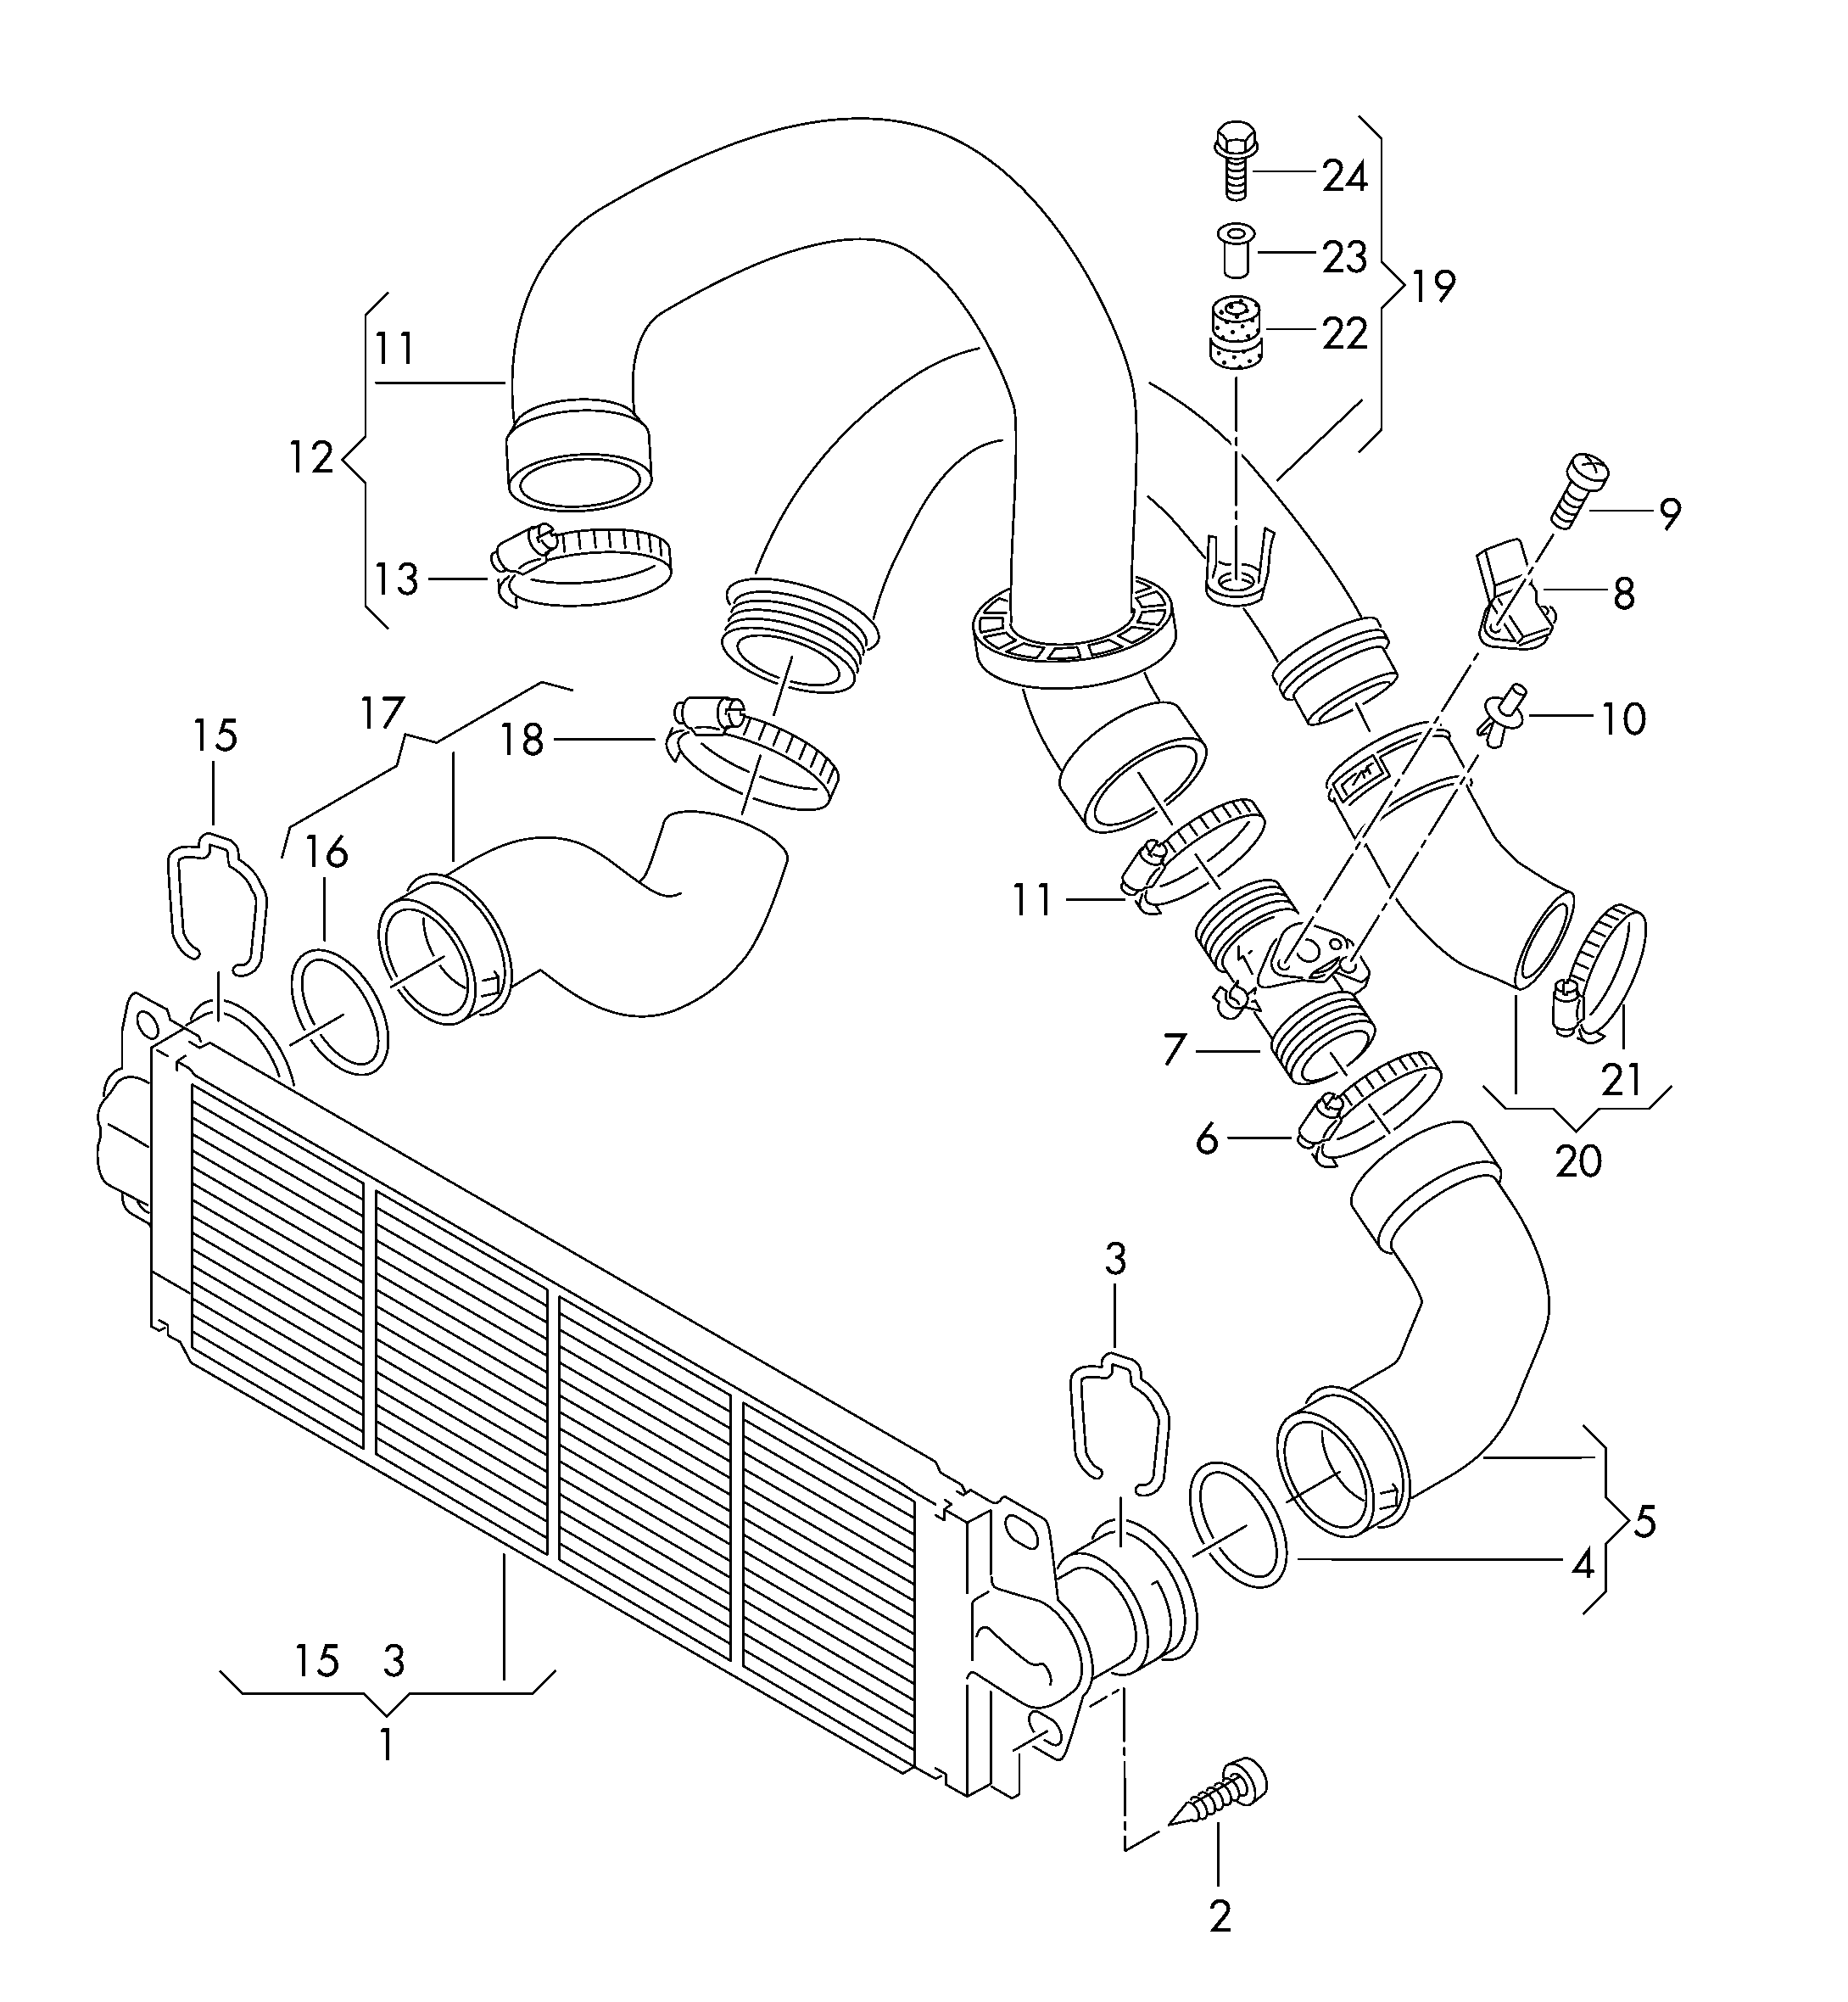
\includegraphics[width=\textwidth]{Ladeluftkuehler}
		\caption{Ladeluftkühler}
		\label{fig:ladeluftkuehler}
	\end{center}
\end{figure}
Halteklammer (Abb. \ref{fig:ladeluftkuehler} -15-) des Schlauches mit einem Schraubendreher lösen, und die Schraube(Abb. \ref{fig:ladeluftkuehler} -24-) des Druckrohrs entfernen. Danach lässt sich der Schlauch nach oben drehen und neben dem Ansaugrohr verstauen. Wer gerne darüber, auf dem Wasserkasten, Schrauben ablegt - besser den Schlauch mit einen Lumpen verschließen.  
Das Kabel an der oberen Zahnriemenabdeckung aushängen und die Verkleidung mit den Klammern lösen.
 
\newpage
\subsection{Luftfilterkasten ausbauen}
Das Ansaugrohr (Abb. \ref{fig:luftfilerkasten} -22-) am Kasten ausclipsen und rausziehen. Nach dem Lösen der Schraube (Abb. \ref{fig:luftfilerkasten} -11-) ist es möglich den Kasten mit recht viel Kraft nach vorne von der Halterung (Abb. \ref{fig:luftfilerkasten} -14-) zu ziehen. Anschließend Kasten samt Bolzen (Abb. \ref{fig:luftfilerkasten} -9-) nach rechts bewegen und komplett ausbauen. Das Entwässerungsrohr kann dran bleiben.

\begin{figure}[htb]
	\begin{center}
		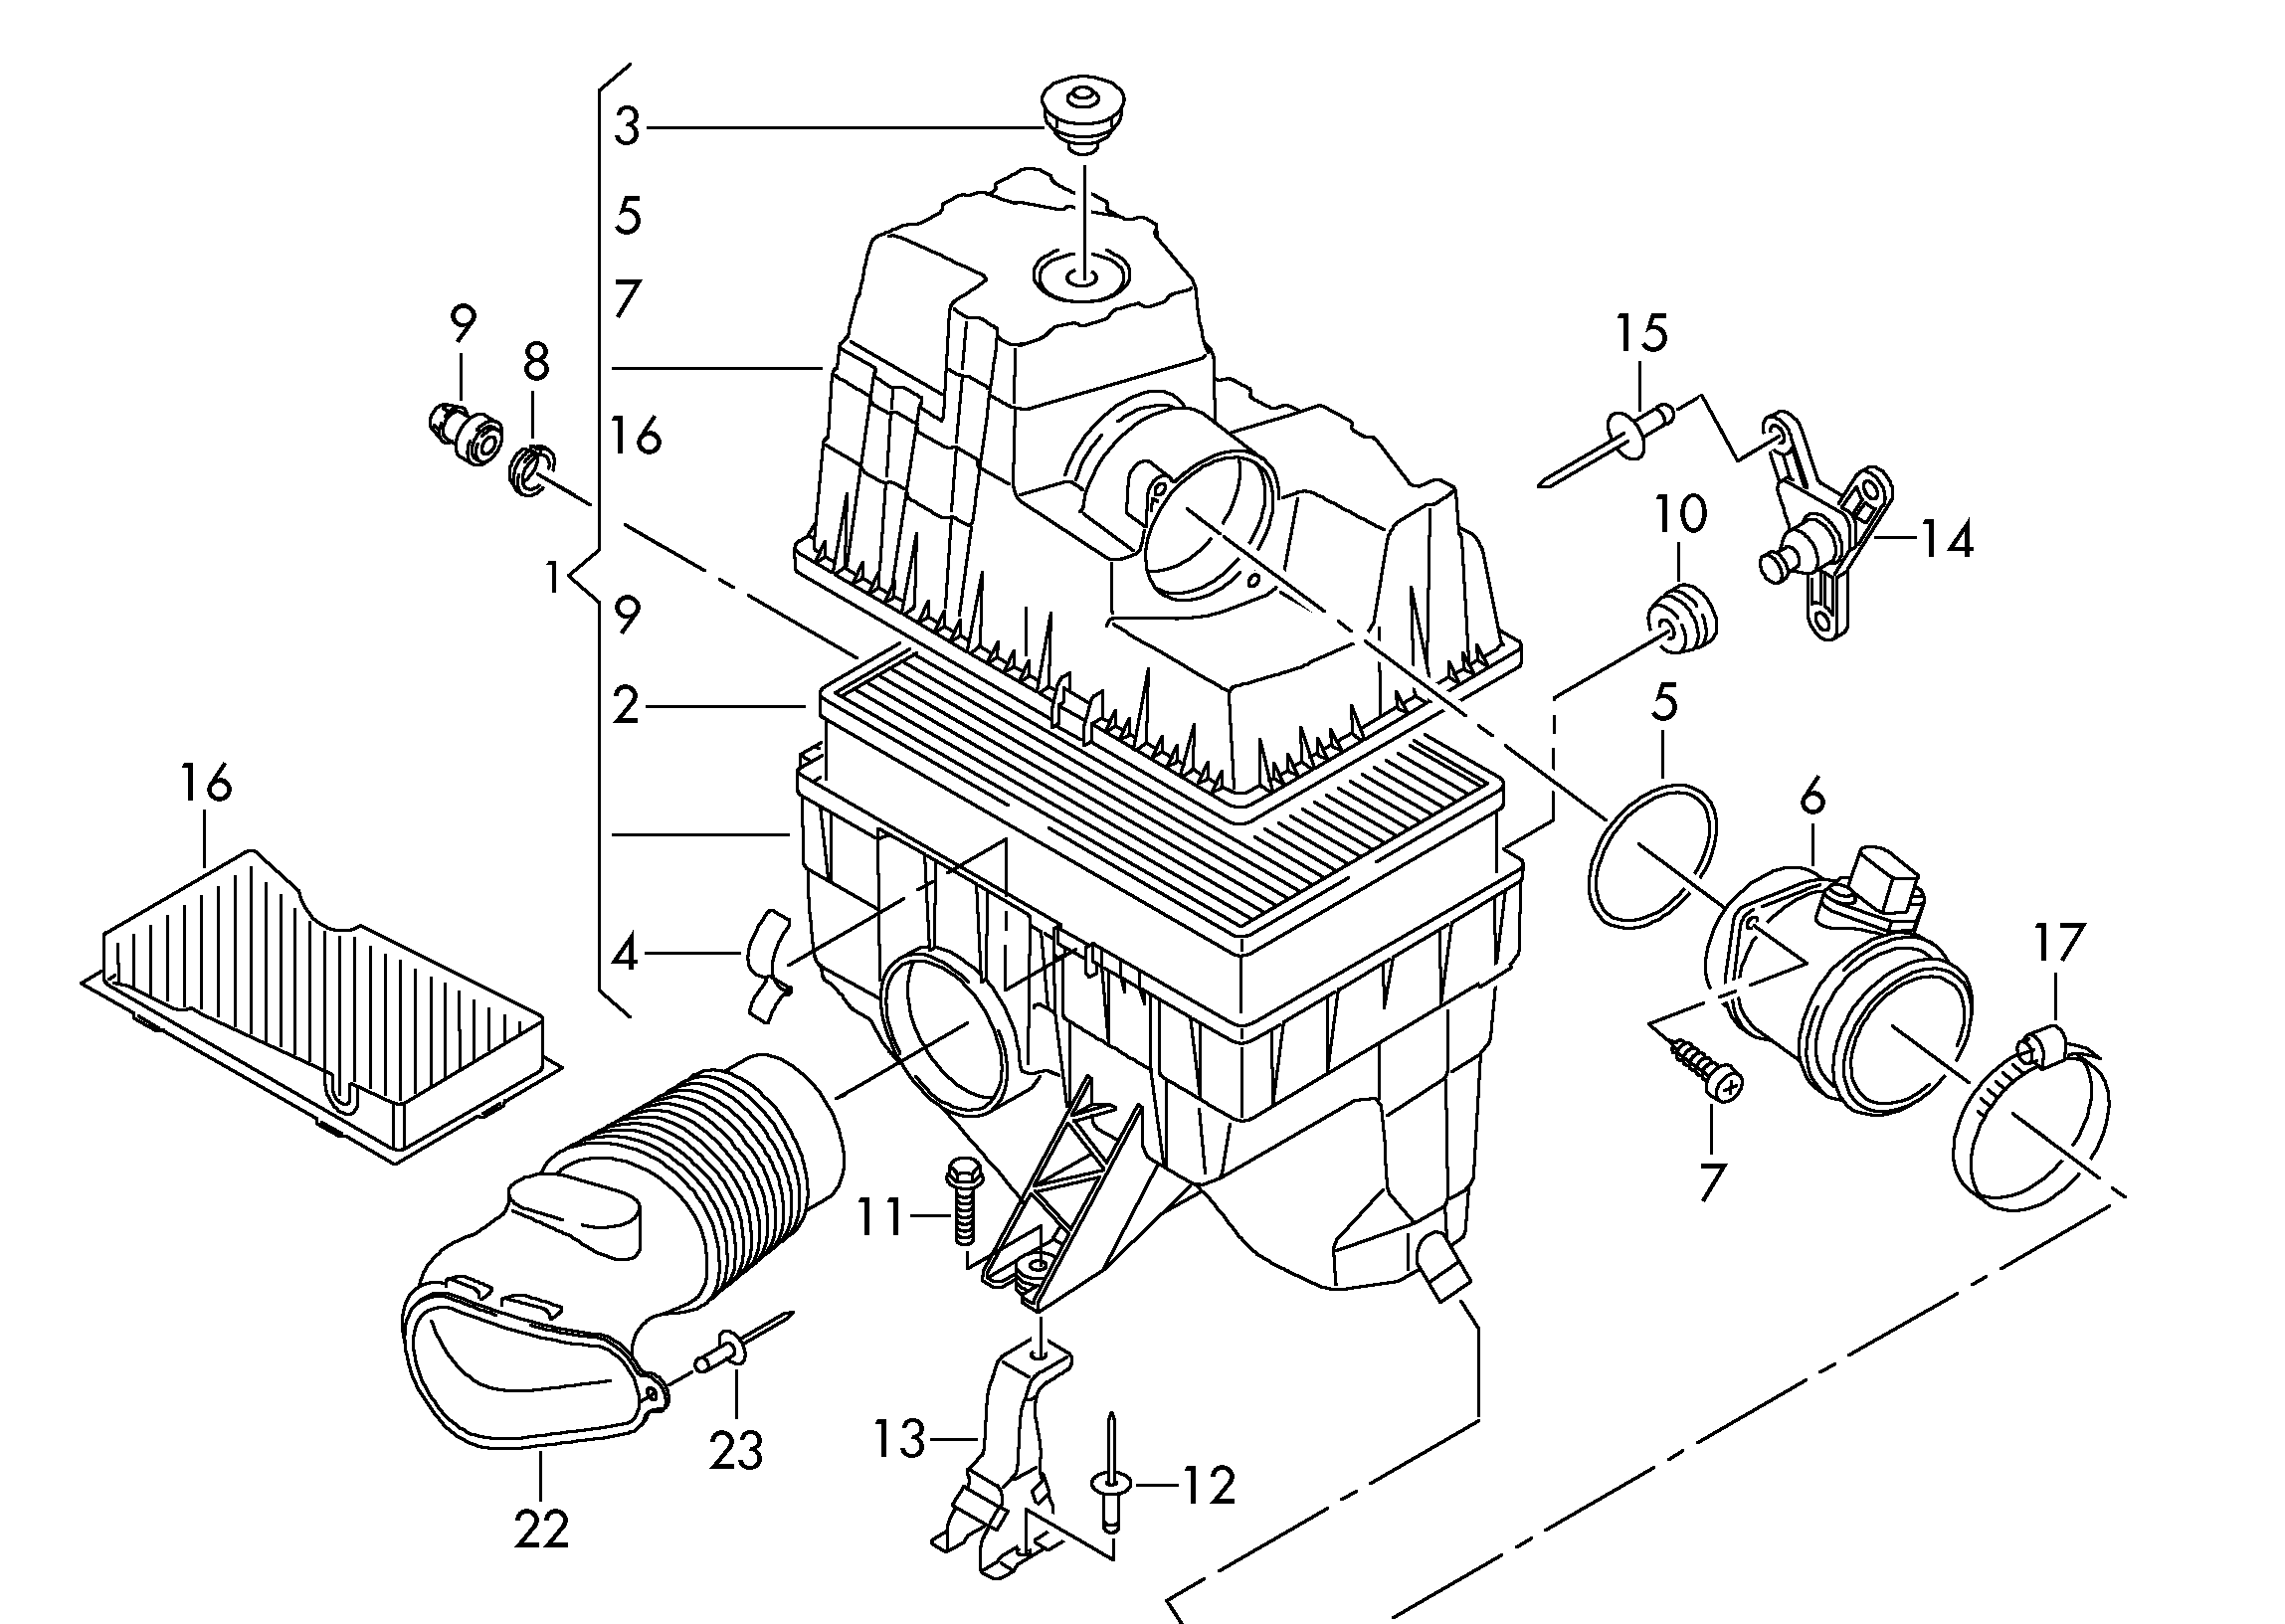
\includegraphics[width=\textwidth]{Luftfilterkasten}
		\caption{Luftfilterkasten}
		\label{fig:luftfilerkasten}
	\end{center}
\end{figure}

\newpage
\subsection{Keilrippenriemen \& Schwingungsdämpfer abbauen}
Der Spanner des Keilrippenriemens mit einem gekröpften 16er Ringschlüssel entspannen und mit einem passenden Stift sichern. Die Laufrichtung der Keilriemens kennzeichnen, z.B. mittels Kreidestift.
Um den Schwingungsdämpfer (Abb. \ref{fig:kurbelwelle} -4-) zu lösen, die vier XZN Schrauben entfernen. Dabei unbedingt an der Zentralschraube mit einem 19er Ringschlüssel gegenhalten. Da ich alleine war, habe ich den Ringschlüssel mit einem Spanngurt am Träger darüber befestigt. Sollte der Schwingungsdämpfer auf der Welle festsitzen hilft ein wenig WD40 (oder gegebenfalls auch der Einsatz eines Schonhammers).

\begin{figure}[htb]
	\begin{center}
		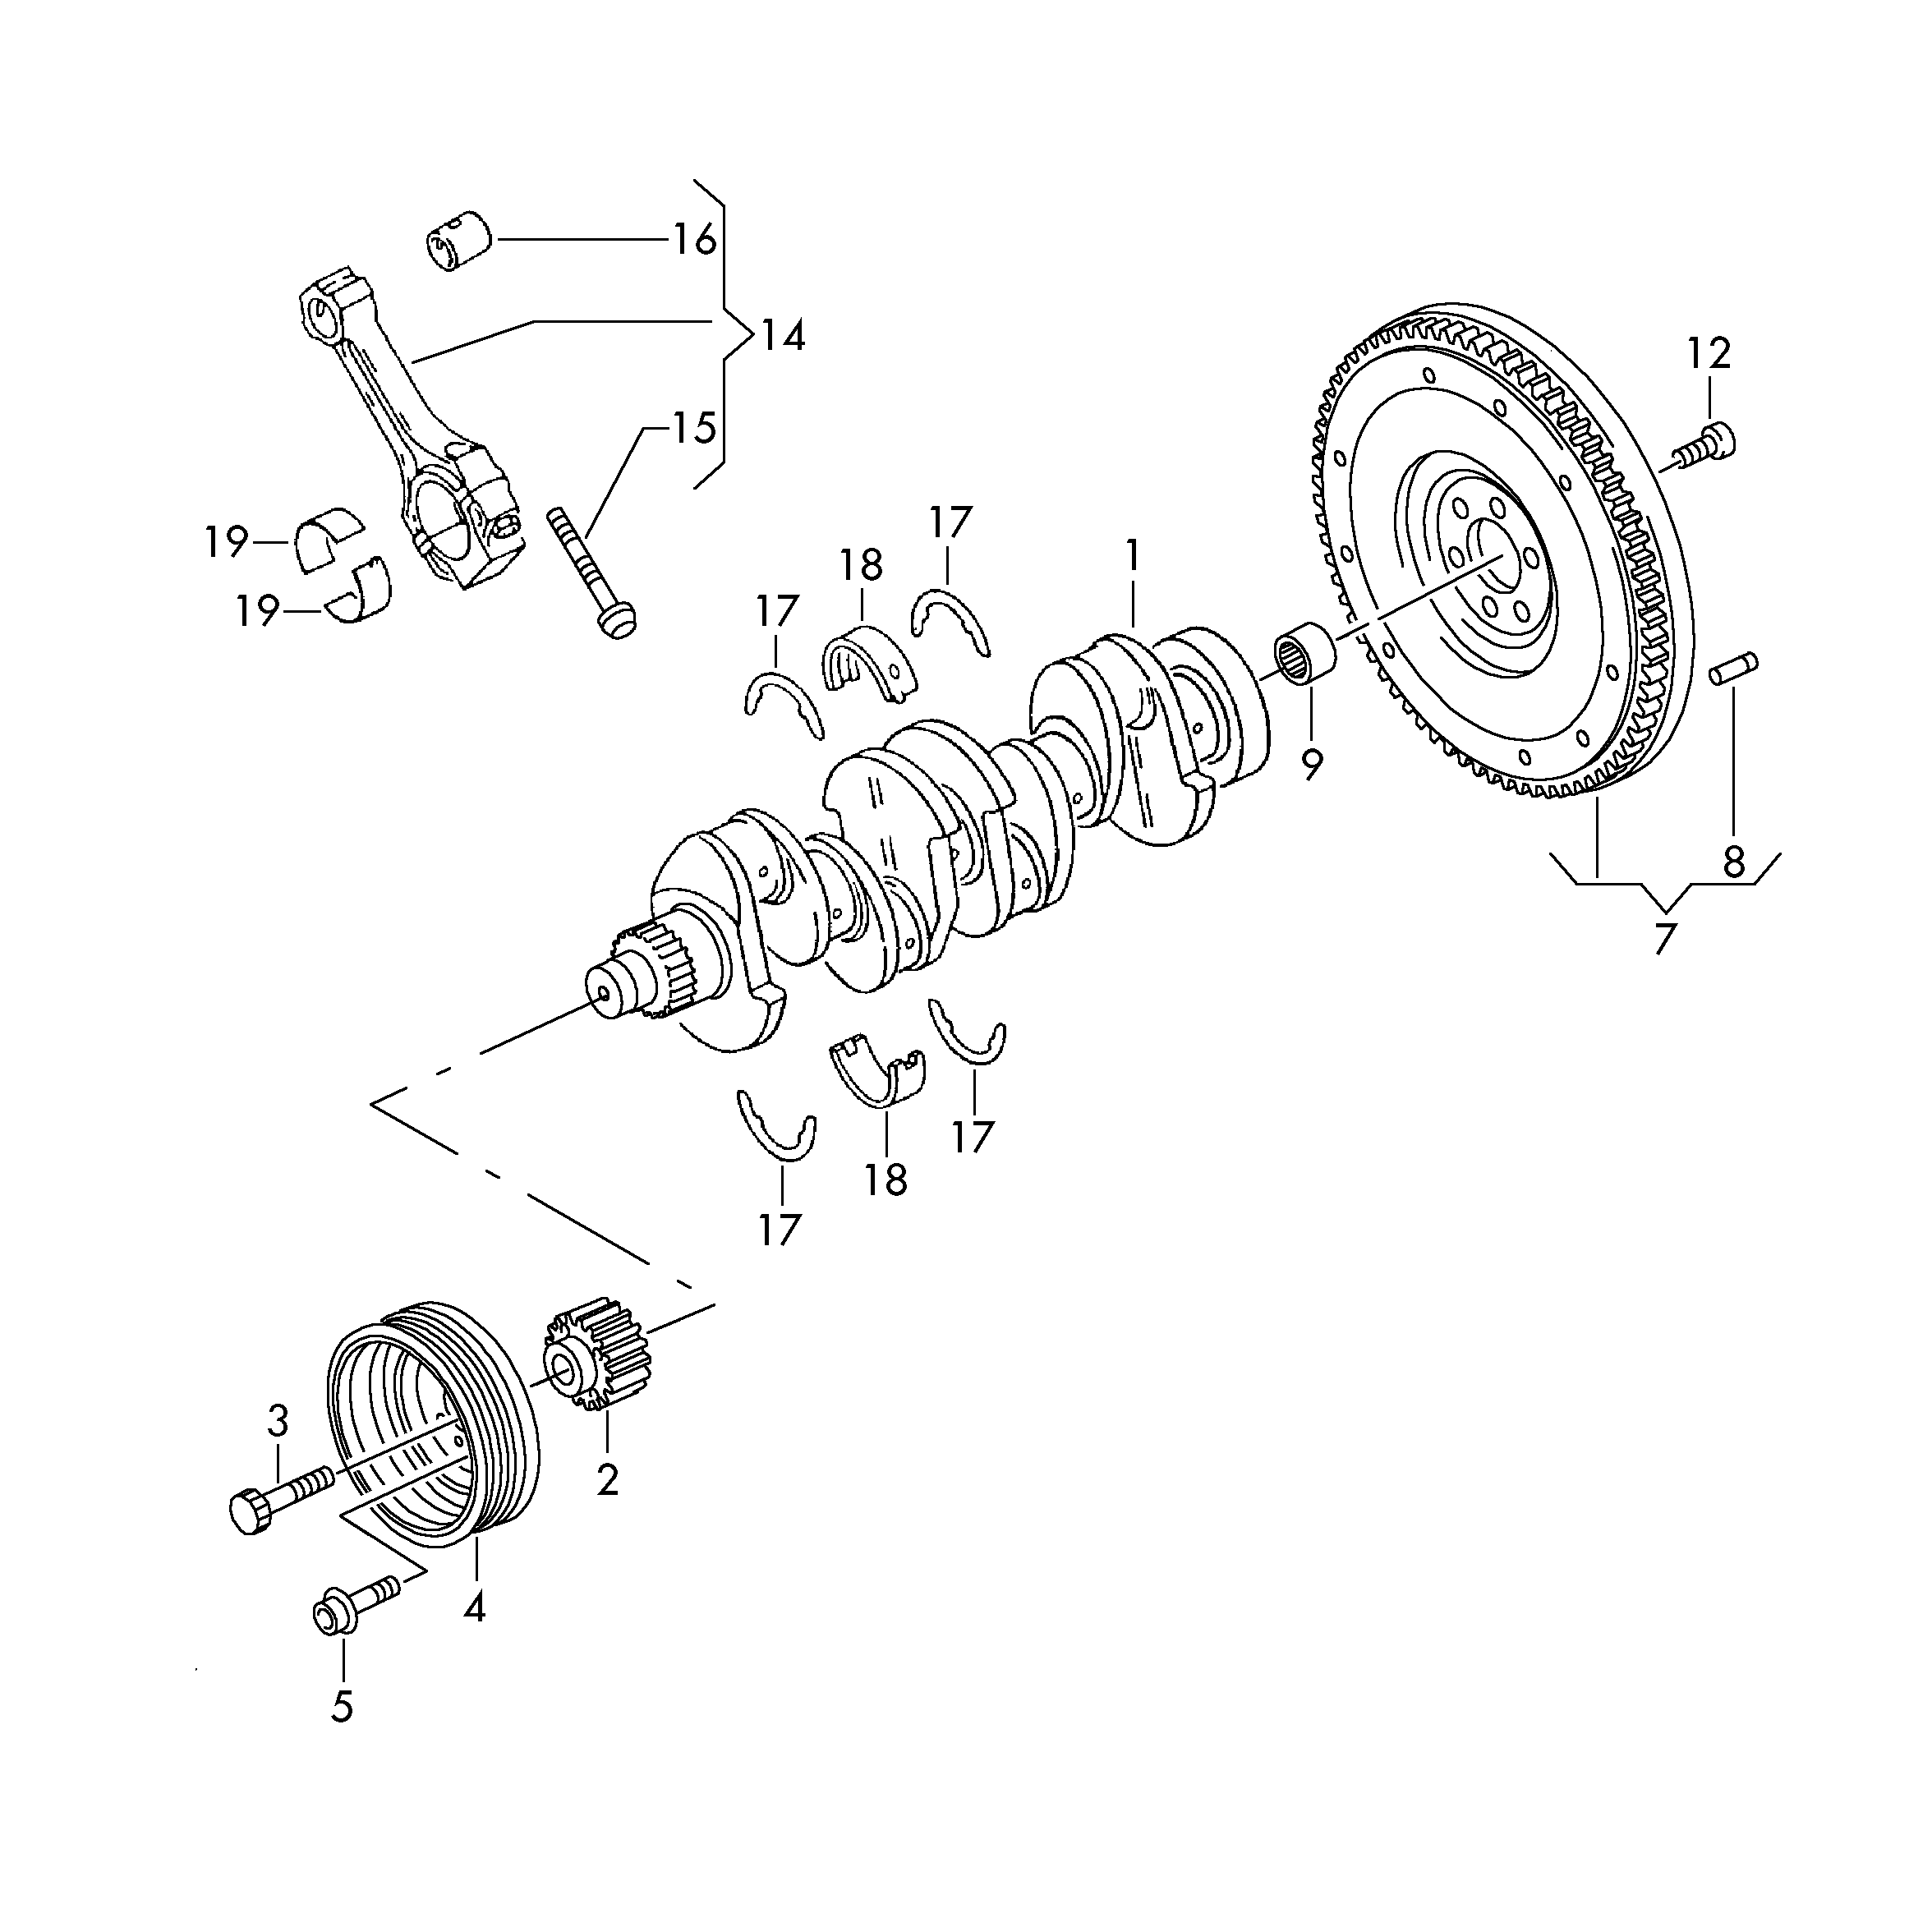
\includegraphics[width=\textwidth]{Kurbelwelle}
		\caption{Kurbelwelle}
		\label{fig:kurbelwelle}
	\end{center}
\end{figure}
\marginlabel{Kommentar:}
Die vier Schrauben (Abb. \ref{fig:kurbelwelle} -5-) müssen beim Zusammenbau ersetzt werden.

\newpage
\subsection{Motorstütze abbauen}
Wenn der Motor sicher abgestützt ist, kann nun die Motorstütze ausgebaut werden. Um die Schrauben leichter zu lösen bietet es sich an, den Motor mit dem Wagenheber minimal anzuheben.
\begin{figure}[htb]
	\begin{center}
		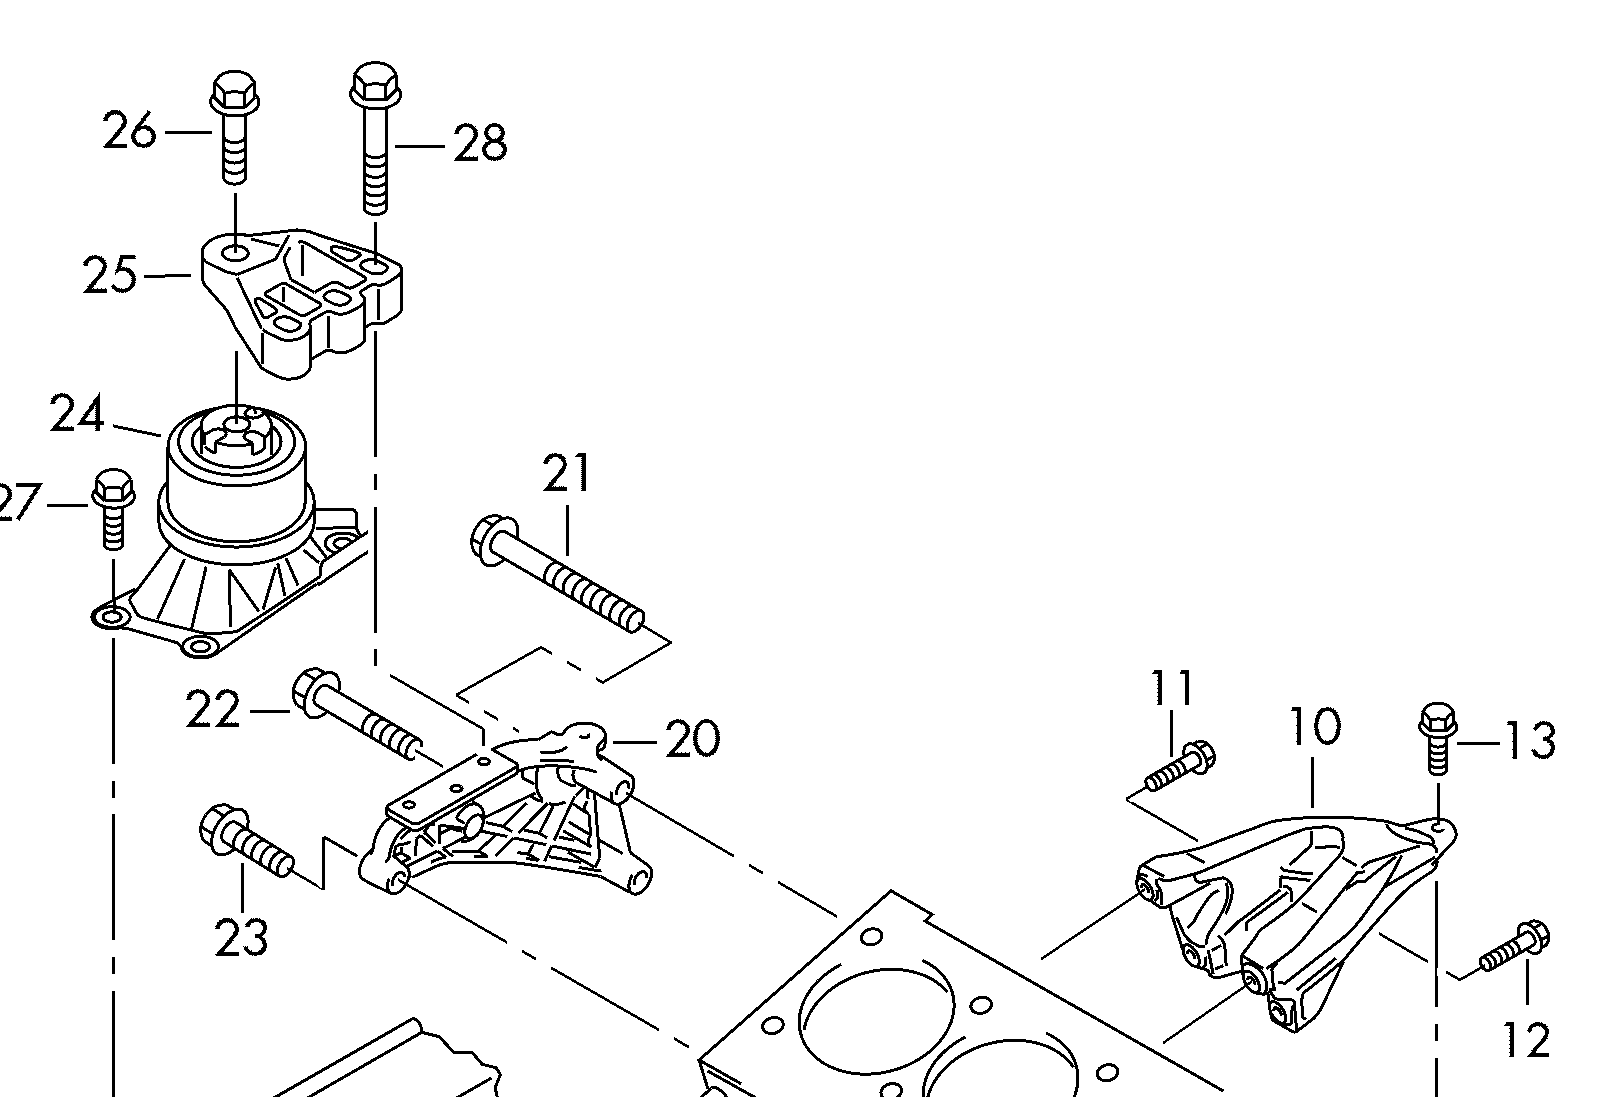
\includegraphics[width=\textwidth]{Motorhalter}
		\caption{Motorhalter}
		\label{fig:motorhalter}
	\end{center}
\end{figure}

\marginlabel{Kommentar:}
Die sieben Schrauben (Abb. \ref{fig:motorhalter} -21- -22- -23- -26- -28-) müssen beim Zusammenbau ersetzt werden.

\newpage
\subsection{Zahnriemenschutz abnehmen}
Den Zahnriemenschutz mit fünf Torx Schrauben entfernen.
\begin{figure}[htb]
	\begin{center}
		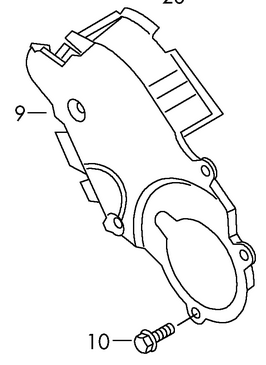
\includegraphics[width=\textwidth]{Zahnriemenabdeckung}
		\caption{Zahnriemenschutz}
		\label{fig:zahnriemenschutz}
	\end{center}
\end{figure}

\newpage

\section{Zahnriemen demontieren}
\subsection{Motor abstecken}
Den Motor in Drehrichtung (im Uhrzeigersinn) drehen, bis die OT Markierung auf dem Nockenwellenrad oben auf kurz vor 12 Uhr steht. \textbf{Dabei immer nur an der Kurbelwelle und in Motor-Drehrichtung drehen!}

Jetzt die Nockenwelle abstecken. Dazu die Kurbelwelle langsam so weit drehen, bis der Absteckdorn ganz einrastet.

Anschließend die Kurbelwelle abstecken(Abb. \ref{fig:KurbelwelleAbstecken}), dazu sollte maximal 1mm Korrektur nötig sein. Das Werkzeug muss ohne verkanten von vorne auf das Zahnrad geschoben werden.

Den Dorn der Nockenwelle wieder entnehmen, die drei Schrauben lösen aber nicht entfernen. Dabei mit dem Gegenhalter arbeiten.

Ebenfalls mit Gegenhalten die drei Schrauben der Hochdruckpumpe lösen aber nicht entfernen.

Die Spannrolle lösen.

Danach die Nockenwelle und die Hochdruckpumpe abstecken.

Jetzt sind Kurbelwelle, Nockenwelle und Hochdruckpumpe fixiert.
\begin{figure}[htb]
	\begin{center}
		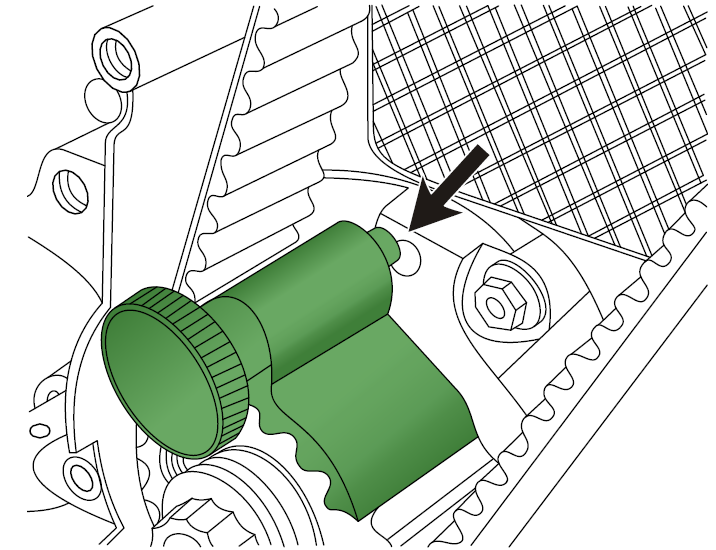
\includegraphics[width=\textwidth]{KurbelwelleAbstecken}
		\caption{Absteckwerkzeug Kurbelwelle}
		\label{fig:KurbelwelleAbstecken}
	\end{center}
\end{figure}


\subsection{Zahnriemen abnehmen}
Ist die Kurbelwelle fixiert, so kann der Zahnriemen abgenommen werden. Vom Nockenwellenrad ausgehend den Riemen schrittweise rundherum abziehen. Gegebenenfalls kann es helfen eine der Umlenkrollen oder die Spannrolle schon auszubauen.

\section{Wasserpumpe und weitere Teile austauschen}
\subsection{Wasserpumpe}
Die Wasserpumpe ist mit 3 Schrauben gesichert. Nach dem Lösen selbiger kann die Wasserpumpe sanft aber bestimmt durch leichtes Wackeln aus ihrem Sitz gezogen werden.
 
Im nächsten Schritt alle Rollen und die zugehörigen Schrauben bzw. Stehbolzen tauschen. Um die Stehbolzen zu entfernen, zwei Muttern M8 aufschrauben und kontern damit  der Stehbolzen entfernt werden kann.
Anzugsmomente für die neuen Rollen/Schrauben in Abbildung \ref{fig:zahnriemen}:
\begin{itemize}
	\item Schraube -22- 10Nm
	\item Bolzen -16- 15Nm?
	\item Schraube -25- 50Nm + $90^\circ$
	\item Bolzen -19- 10Nm?
	\item Mutter -20- 20Nm
\end{itemize}
\begin{figure}[htb]
	\begin{center}
		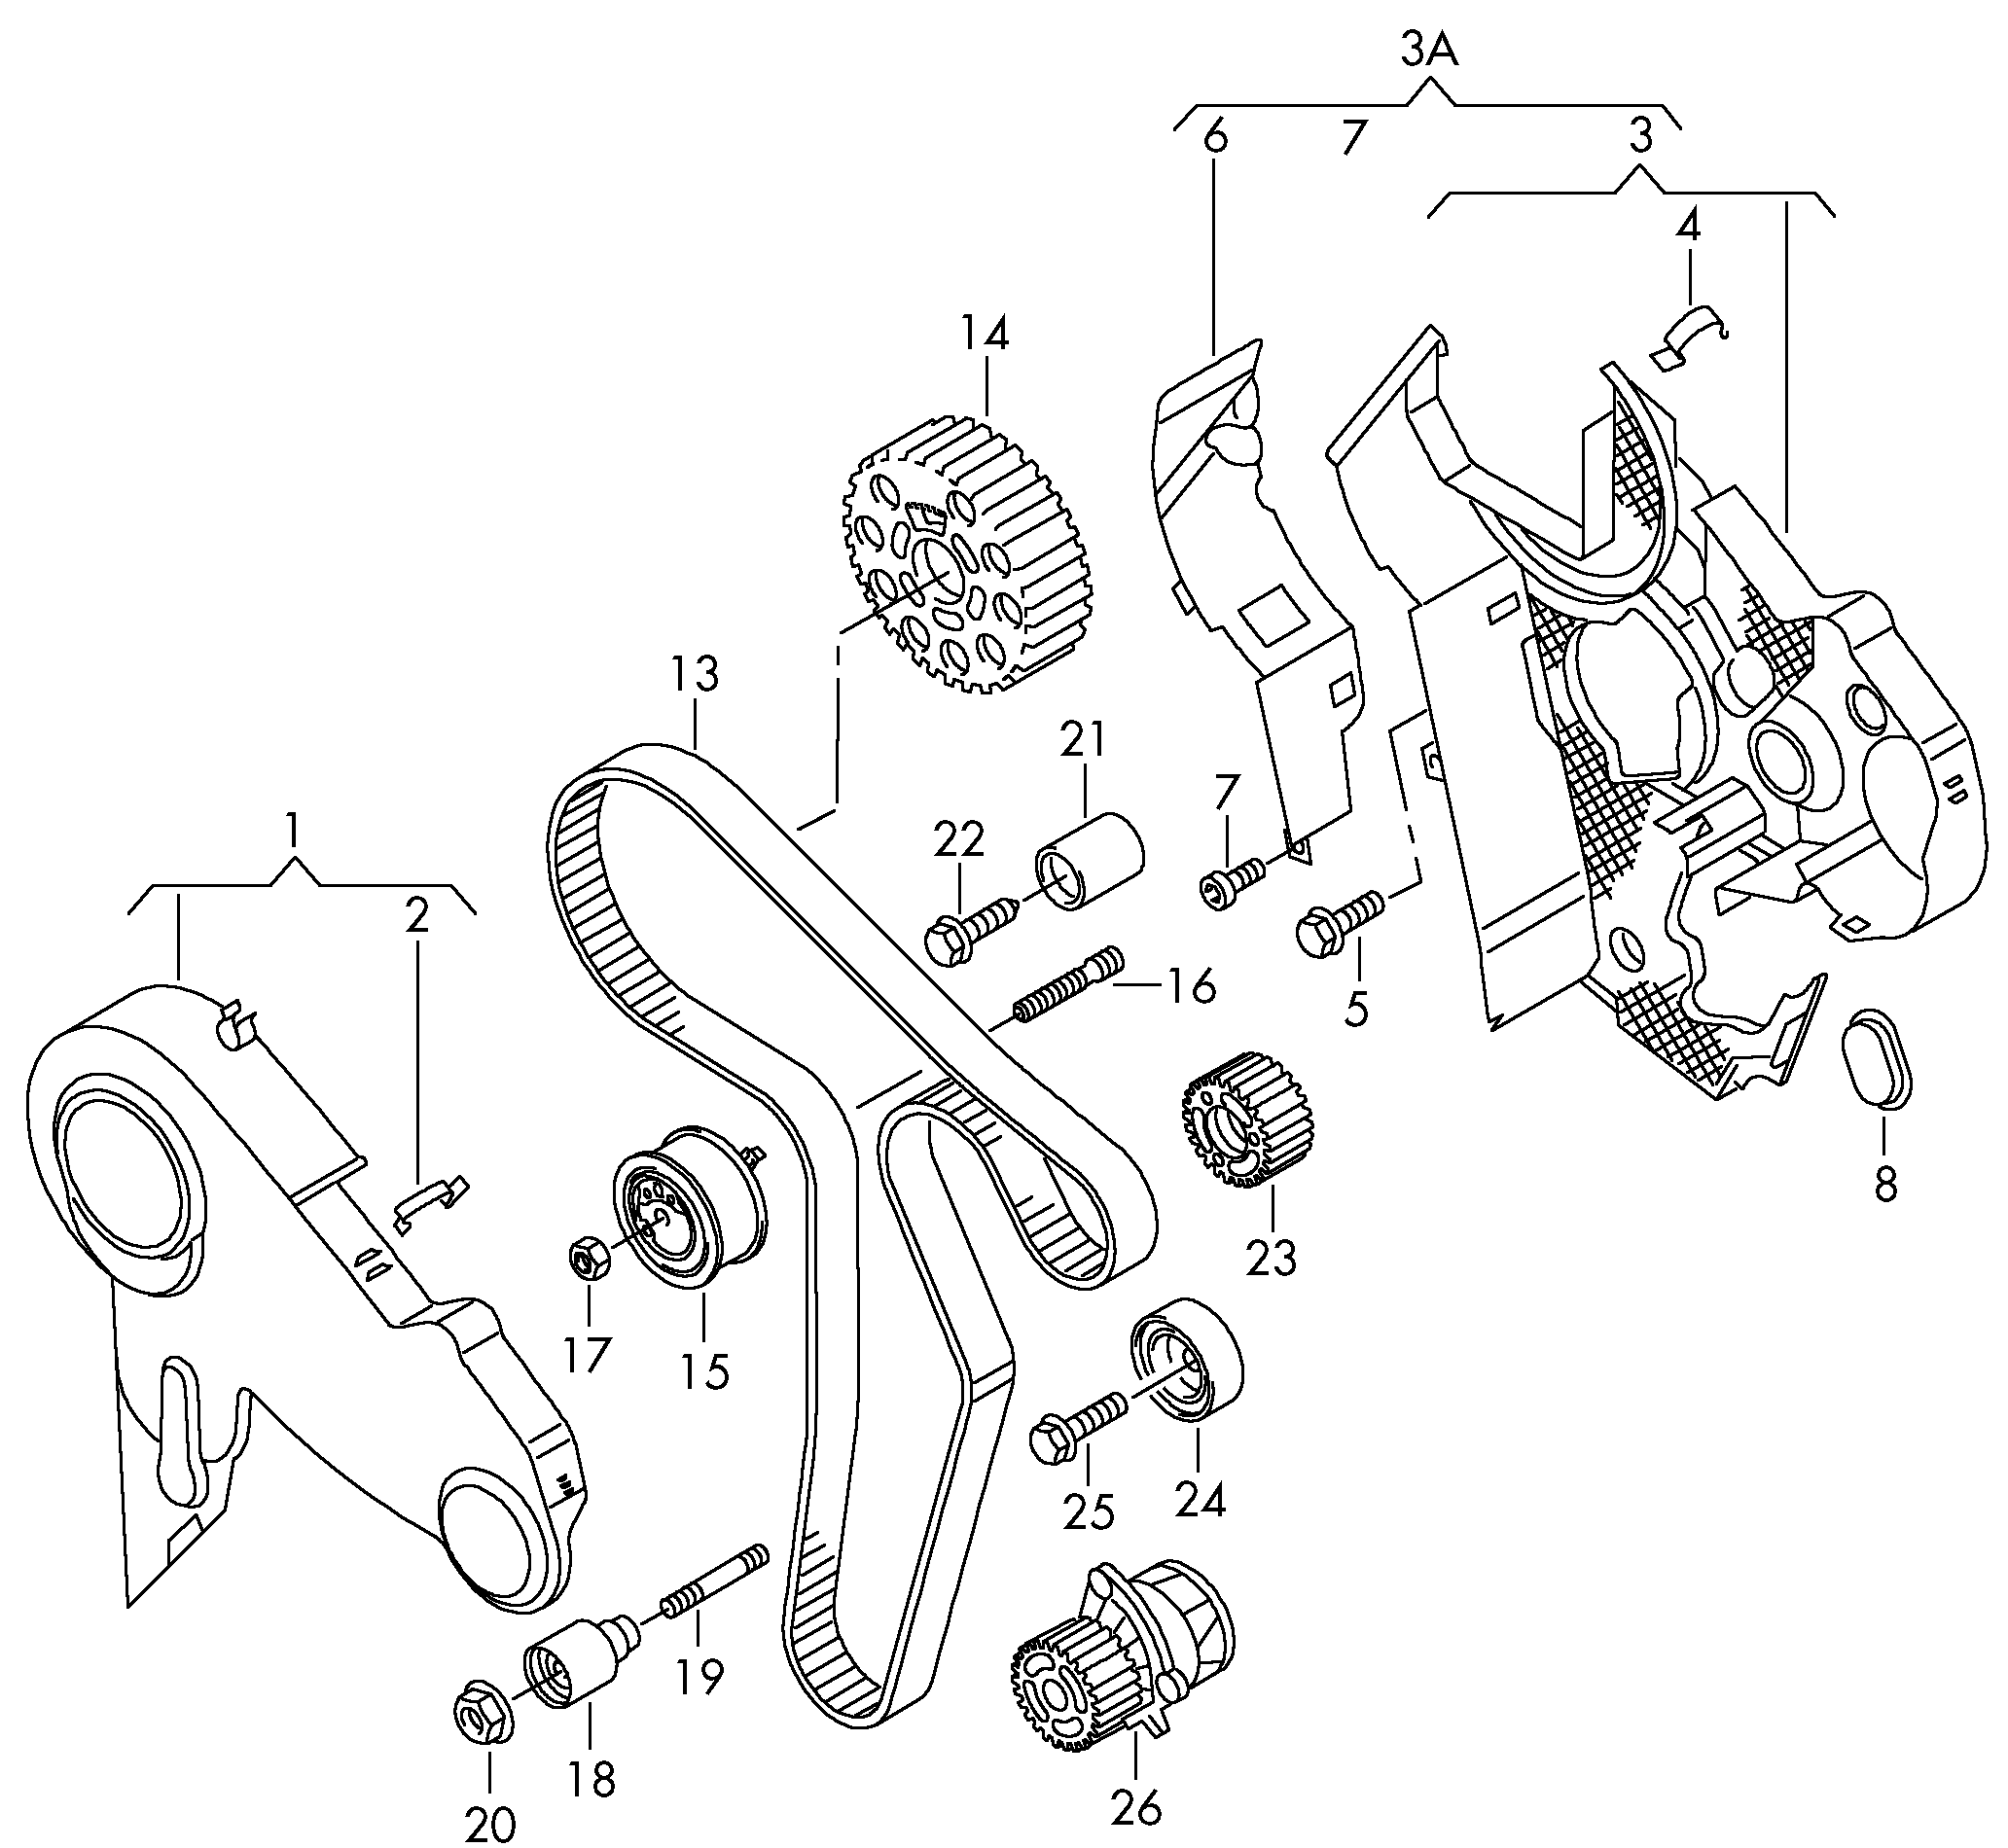
\includegraphics[width=\textwidth]{Zahnriemen}
		\caption{Zahnriemen, Umlenkrollen etc.}
		\label{fig:zahnriemen}
	\end{center}
\end{figure}
Vor dem Einsetzen der neuen Wasserpumpe den Sitz der Pumpe am Motor säubern und den Dichtring mit frischem Kühlmittelkonzentrat benetzen, um die Montage zu vereinfachen. Die Wasserpumpe platzieren und mit den drei Schrauben gegen herausfallen sichern. Ich habe die Pumpe leider nicht von Hand in den Sitz geschoben bekommen. Deshalb habe ich die Schrauben ringsum jeweils ein kleines Stück fester gezogen um die Pumpe ohne verkanten und ohne Beschädigung der Dichtung in den Sitz zu drücken. Anzugsmoment der Wasserpumpenschrauben 15\,Nm.

Beim Einsetzen des Spanners -15- darauf achten, dass die Nase richtig in der Bohrung sitzt.

\section{Zahnriemen auflegen}
Der folgende Arbeitschritt wird unter Umständen einige Tropfen Schweiß und den ein oder anderen Fluch kosten. Der neue Zahnriemen ließ sich, zumindest bei mir, nur sehr schwer auflegen.

Nockenwellenrad und das Zahnriemenrad der Hochdruckpumpe in ihren Langlöchen im Uhrzeigersinn auf Anschlag drehen. Damit geht das Auflegen etwas leichter. Dabei darauf achten, dass die Schrauben fest genug sind, dass die Räder kein Kippspiel haben.

Den Zahnriemen in der folgenden Reihenfolge auflegen:
\begin{enumerate}
	\item Kurbelwelle
	\item Spannrolle
	\item Nockenwelle
	\item Kühlmittelpumpe
	\item Hochdruckpumpe
	\item Umlenkrolle
\end{enumerate}
Den Riemen zu Beginn nur vorne auf die entsprechenden Räder auflegen und anschließend gleichmäßig, ohne den Einsatz von Werkzeug, bündig auflegen.

Nun die Spannrolle im Pfeilrichtung (Uhrzeigersinn) spannen und die Mutter mit 20 Nm +  $45^\circ$ fest ziehen.

Die Schrauben des Nockenwellenrades und der Hochdruckpumpe tauschen. Dazu jeweils zwei Schrauben handfest anziehen und die Dritte auswechseln. Anschließend unter Zuhilfenahme des Gegenhalters die Schrauben festziehen. Nockenwellenschrauben 20 Nm +  $45^\circ$, Hochdruckpumpe 20 Nm +  $90^\circ$ .\\
\marginlabel{Kommentar:}
Den endgültigen Drehwinkel der Schrauben erst nach Kontrolle der Steuerzeiten (siehe nächster Abschnitt) einstellen.
\section{Kontrolle}
Sind alle Schrauben festgezogen muss jetzt die Einstellung der Steuerzeiten kontrolliert werden.

Dazu das Absteckwerkzeug entfernen und den Motor an der Kurbelwelle zwei mal durchdrehen. Anschließend müssen sich die Absteckwerkzeuge wieder leicht montieren lassen.

Die Kurbelwelle abstecken. Jetzt muss selbiges bei der Nockenwelle ohne Probleme ebenfalls funktionieren. Auch bei der Hochdruckpumpe sollte dies der Fall sein, laut VW Reparaturleitfaden ist eine geringe Abweichung wie in Abbildung \ref{fig:hdp} zu sehen jedoch unproblematisch.

\begin{figure}[htb]
	\begin{center}
		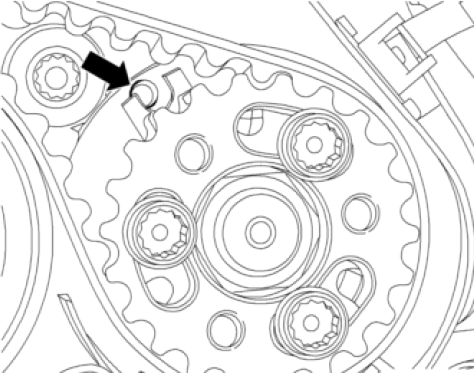
\includegraphics[width=\textwidth]{HDPabweichung}
		\caption{Abweichung der Nullstellung Hochdruckpumpe}
		\label{fig:hdp}
	\end{center}
\end{figure}


Zur Sicherheit das Ganze nochmal... und nochmal ... und wer das zum ersten Mal macht, so wie ich: nochmal - An dieser Stelle muss wirklich alles stimmen!

Wenn alles passt: Drehwinkel der Schrauben an Nockenwellenrad und Hochdruckpumpe einstellen und nochmals die Spannung der Spannrolle sowie alle Schrauben und Muttern des Riementriebs überprüfen.

Für den Fall, dass es nicht so passt wie gewünscht, hier ein Zitat aus dem Reparaturleitfaden:\\
\textit{Lässt sich die Nabe der Nockenwelle nicht arretieren:\\
– Den Kurbelwellenstopp so weit zurückziehen, dass
der Zapfen die Bohrung frei gibt.\\
– Die Kurbelwelle entgegen der Motordrehrichtung etwas über
den oberen Totpunkt hinausdrehen.\\
– Die Kurbelwelle langsam in Motordrehrichtung drehen, bis
sich die Nabe der Nockenwelle abstecken lässt.\\
– Nach dem Abstecken die Schrauben des Zahnriemenrads der
Nockenwelle lösen.\\}


\textit{Steht der Zapfen des Kurbelwellenstopp links neben
der Bohrung:\\
– Die Kurbelwelle in Motordrehrichtung drehen, bis der Zapfen
des Kurbelwellenstopps aus der Drehbewegung heraus in den
Dichtflansch eingreift.\\
– Schrauben des Zahnriemenrads der Nockenwelle zunächst
handfest anziehen und anschließend festziehen.\\}


\textit{Steht der Zapfen des Kurbelwellenstopp rechts neben
der Bohrung:\\
– Die Kurbelwelle wieder etwas entgegen der Motordrehrichtung
drehen.\\
– Jetzt die Kurbelwelle in Motordrehrichtung drehen, bis der
Zapfen des Kurbelwellenstopps aus der Drehbewegung heraus
in den Dichtflansch eingreift.\\
– Schrauben des Zahnriemenrads der Nockenwelle zunächst
handfest anziehen und anschließend festziehen.}

\section{Zusammenbau}
Zum Abschluss alles in umgekehrter Reihenfolge wieder zusammenbauen.
Anzugsmomente für die neuen Schrauben des Motorhalters in Abbildung \ref{fig:motorhalterschrauben}:
\begin{itemize}
	\item Schraube -26- 90Nm + $90^\circ$
	\item Schrauben -28- 50Nm + $90^\circ$
	\item Schraube -21/22/23- 40Nm + $90^\circ$
\end{itemize}
\begin{figure}[htb]
	\begin{center}
		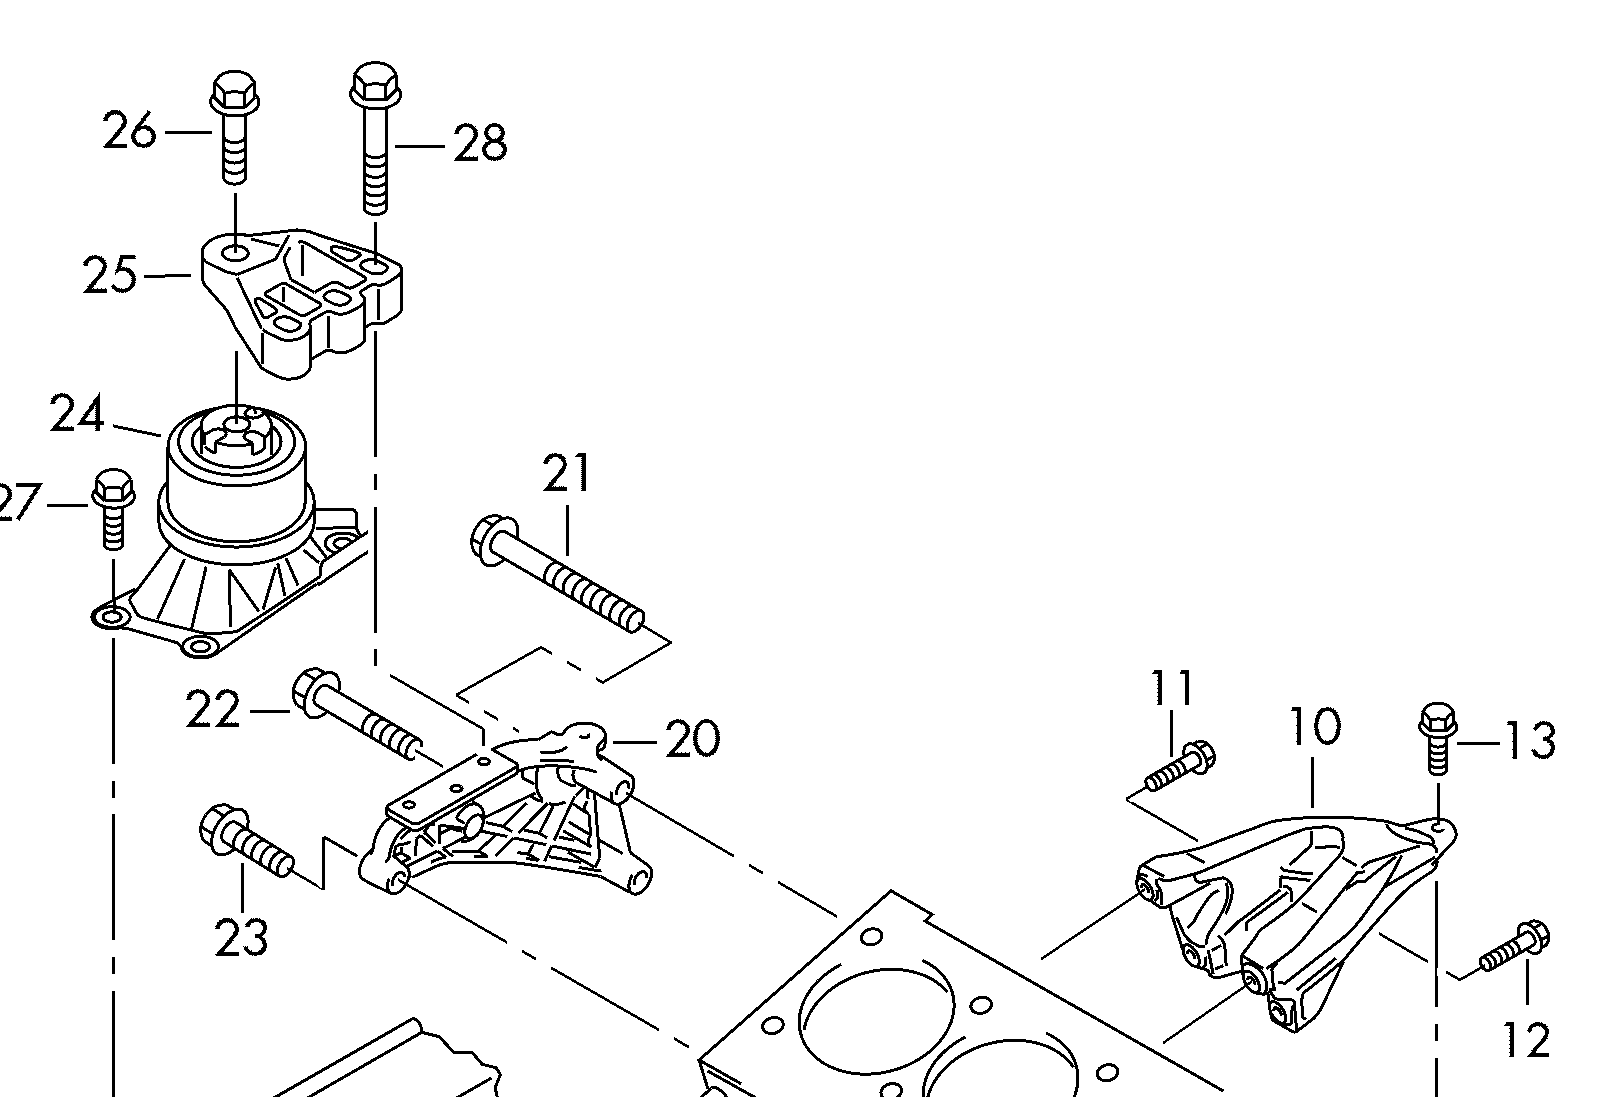
\includegraphics[width=\textwidth]{Motorhalter}
		\caption{Motorhalter}
		\label{fig:motorhalterschrauben}
	\end{center}
\end{figure}
Die Riemenscheibe des Keilrippenriemen mit neuen Schrauben montieren 10Nm + $90^\circ$.

Kühlwasser auffüllen, insgesamt gehen so ca. 9L rein.

\section{Motor starten}
Der Moment der Wahrheit - wenn alles passt kann der Motor nun wieder gestartet werden.
Um den Kühlkreislauf zu entlüften den Motor für ca. 3 Minuten auf 2000 U/min halten. Dabei das Kühlmittel nachfüllen.

Mittels VCDS kann bei kaltem Motor der Verdrehwinkel überprüft werden:\\ Nockenwellenadaption Einlass Bank 1: Phasenlage\\
Dieser sollte möglichst nah an $0^\circ$ liegen.

%%%%%%%%%%%%%%%%%%%%%%%%%%%%%%%%%%%%%%%%%%%%%%%%%%%%%%%%%%%%%%%%%%%%%%

\printindex

\end{document}
